\section{Introduction}


\subsection{Summarization}

\begin{frame}{Summarization Overview}

\begin{itemize}
  \item \textbf{Definition} Summarization involves condensing natural language
	while retaining essential information for quicker readability and interpretation.
	\item<2-> \textbf{Importance} Summarization is crucial because it helps us extract
	important information efficiently.
	\item<3-> \textbf{Role for long texts} Summarization can be a valuable tool with
	long texts that can let us decide whether the whole text is worth reading.
\end{itemize}

\vskip .5cm

\begin{figure}
	\centering
	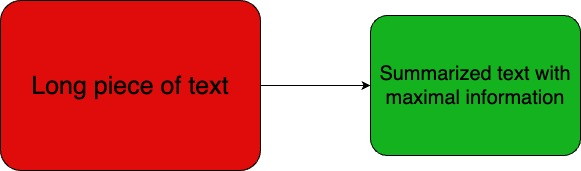
\includegraphics[width=.8\textwidth]{Images/summarize.jpg}
\end{figure}

\end{frame}


\subsection{Automatic Summarization}

\begin{frame}{What's Automatic Summarization?}

Summarization done by a computer algorithm automatically is known as automatic
summarization.

\begin{itemize}
	\item<2-> \textbf{Extractive methods} These methods focus on selecting/extracting
	key sentences or phrases from the text.
	These selected phrases are combined to form the summary.
	\item<3-> \textbf{Abstractive methods} These methods generate the summary from
	scratch using state-of-the-art NLP algorithms.
	Abstractive methods generally produce better results than extractive methods but
	are computationally extensive.
\end{itemize}

\vskip .5cm

\begin{figure}
	\centering
	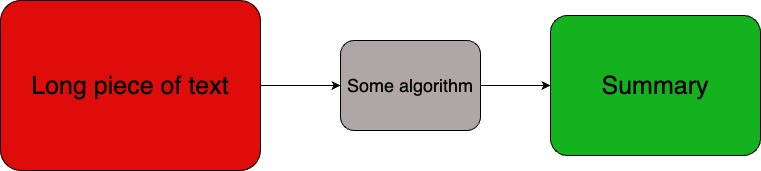
\includegraphics[width=.9\textwidth]{Images/algorithm-summarize.jpg}
\end{figure}

\end{frame}

\begin{frame}{How is it done today?}

Nowadays, we have sophisticated Large Language Models (LLMs) based on the
transformer architecture for automatic summarization.
These methods have pushed the boundaries of abstractive summarization and can
generate accurate, coherent, and human-like summaries.

\only<1>{
	\vskip 2.63cm
}

\vskip 1.3cm

\only<2>{
	\begin{figure}
		\centering
		
\includegraphics[width=.2\textwidth]{Images/GPT-4.png}
		\hfill
		
\includegraphics[width=.4\textwidth]{Images/bert.jpg}
		\hfill
		
\includegraphics[width=.35\textwidth]{Images/llama.jpg}
	\end{figure}
}

\end{frame}
